\documentclass[a4paper,12pt,parskip,bibtotoc,liststotoc]{article}
    %Festlegung der Dokumentenklasse, zahlreiche Vereinbarungen über Layout, Gliederungsstrukturen,
    %bsp. article -> section, subsection..., book -> chapter, section...
    %parskip = Abstand zwischen Absätzen, Veränderung durch \setlength

\usepackage[ngerman]{babel}     %Neue deutsche Rechtschreibung, Umlaute können geschrieben werden
\usepackage[utf8]{inputenc}     %direkte Angabe von Umlauten
\usepackage[T1]{fontenc}        %Silbentrennung bei Sonderzeichen
\usepackage{setspace}           %für Zeilenabstand
\usepackage[notindex,nottoc]{tocbibind}   %Inhaltsverzeichnisse erstellen


\usepackage{mathptmx,charter,courier} % Für schöne Schriften
\usepackage[scaled]{helvet}     		%Serifenlose Schrift wird in Helvetica geschrieben
\usepackage{calligra}    				%Calligra Schriftart
\usepackage{eufrak}      				%mathematische Symbole


%zusätzliche benötigte Pakete
\usepackage{graphicx}           %Graphik
\usepackage{amsmath}    		%Mathematik
\usepackage{natbib}             %Zitate
\usepackage{marvosym}           %enthält Symbole wie das Eurozeichen
\usepackage{eurosym}

%\setcounter{secnumdepth}{3}
%\setcounter{tocdepth}{3}



\usepackage{mdwlist}   			%Verringerung Abstand zwischen items -> \begin{itemize*} \end{itemize*}
\usepackage[labelsep=space,justification=centering]{caption} % Abbilungd-/Tabellen Über-/Unterschriften

%\usepackage{hyperref}  		%erlaubt Links innerhalb des pdf-Dokuments zu erzeugen

\setlength{\parindent}{0pt}     %Verhinderung des horizontalen Einrückens zu Beginn eines Absatzes

%Seitenlayout
\topmargin -0.9cm       %Vertikaler Abstand der Kopfzeile von der Bezugslinie
\textheight 25cm        %Abstand der Grundlinie der Kopfzeile zum Haupttext
\textwidth 16.5cm       %Breite des Haupttexts
\footskip 1cm           %Abstand der Grundlinien der letzten Textzeile und der Fußzeile
\voffset -0.5cm         %Vertikale Bezugspunktposition
\hoffset -1.2cm         %Horizontale Bezugspunktposition

\onehalfspacing         %anderthalbzeiliger Abstand

\newcommand{\url}{\;}   %URL im Literaturverzeichnis

%eigene Befehlsdefinitionen
\newcommand{\be}{\begin{equation}}     %Mathematische Umgebung
\newcommand{\ee}{\end{equation}}
\newcommand{\bea}{\begin{eqnarray}}
\newcommand{\eea}{\end{eqnarray}}
\newcommand{\bean}{\begin{eqnarray*}}  %ohne Nummerierung
\newcommand{\eean}{\end{eqnarray*}}    %ohne Nummerierung

%%%%%%%%%%%%%%%%%%%%%%%%%%%%%%%%%%%%%%%%%%%%%%%%%%%%%%
%
%    Anfang des Textes
%
%%%%%%%%%%%%%%%%%%%%%%%%%%%%%%%%%%%%%%%%%%%%%%%%%%%%%%
\begin{document}

\pagenumbering{roman}  %römische Seitennummerierung
%%%%%%%%%%%%%%%%%%%%%%%%%%%%%%%%%%%%%%%%%%%%%%%%%%%%%%
%
%    Titelseite
%
%%%%%%%%%%%%%%%%%%%%%%%%%%%%%%%%%%%%%%%%%%%%%%%%%%%%%%
\thispagestyle{empty}  %keine Seitenzahl auf Titelseite
Leibniz Universität Hannover\\
Wirtschaftswissenschaftliche Fakultät\\
Institut für Produktionswirtschaft\\
Prof.\ Dr.\ Stefan Helber

\vspace{5cm}

\begin{center}
Hausarbeit \\
im Rahmen des Seminars zur Produktionswirtschaft im WS 2016/17 \\
(Veranstaltungs-Nr. 171137)

\vspace{2.5cm}

Thema Nr. ..\\[1mm]    %hier Themennummer eintragen
{\Large Titel }
\end{center}

\vspace{7.5cm}

Vorname Name \\
Straße Hausnummer \\
PLZ Ort \\
Matr.-Nr. 1234567 \\[3mm]
Abgabedatum:


\newpage

%Inhaltsverzeichnis erstellen
\tableofcontents

\newpage  %neue Seite

%Abbildungsverzeichnis erstellen
\listoffigures

%Tabellenverzeichnis erstellen
\listoftables

%Abkürzungsverzeichnis
\section*{Abkürzungsverzeichnis}
\addcontentsline{toc}{section}{Abkürzungsverzeichnis}
\begin{table}[h!]
    \vspace*{-3mm}
    \hspace*{2mm}
  \renewcommand{\arraystretch}{1,5}
    \begin{tabular}{ll}  %hier die Spaltenausrichtung und Anzahl eintragen
     LP	        & Linear Programming\\
     MIP		& Mixed Integer Programming\\
     OR		    & Operations Research\\
     RCPSP      & Resource-Constrained Project Scheduling Problem\\
     TSP        & Traveling Salesman Problem\\
     WYSIWYG    & What You See Is What You Get\\
     WYSIWYM    & What You See Is What You Mean\\
	\end{tabular}
\end{table}

%Symbolverzeichnis
\section*{Symbolverzeichnis}
\addcontentsline{toc}{section}{Symbolverzeichnis}
\begin{table}[h!]
    \vspace*{-3mm}
    \hspace*{2mm}
  \renewcommand{\arraystretch}{1,5}
    \begin{tabular}{ll}  %hier die Spaltenausrichtung und Anzahl eintragen
     $\alpha$	& alpha\\     %hier $-Operatoren verwenden, da mathematischer Ausdruck im Text
	\end{tabular}
\end{table}

\newpage

\pagenumbering{arabic}   %ab hier arabische Seitenzahlen beginnend mit 1
%%%%%%%%%%%%%%%%%%%%%%%%%%%%%%%%%%%%%%%%%%%%%%%%%%%%%%
%
%   1  Einleitung
%
%%%%%%%%%%%%%%%%%%%%%%%%%%%%%%%%%%%%%%%%%%%%%%%%%%%%%%
\section{Einleitung}

%%%%%%%%%%%%%%%%%%%%%%%%%%%%%%%%%%%%%%%%%%%%%%%%%%%%%%
%
%    hier Titel des nächsten Kapitels eingeben
%
%%%%%%%%%%%%%%%%%%%%%%%%%%%%%%%%%%%%%%%%%%%%%%%%%%%%%%
\section{Grundlagenteil}

%Hier steht kein Text, wenn ein Unterpunkt folgt!\\\\

%%%%%%%%%%%%%%%%%%%%%%%%%%%%%%%%%%%%%%%%%%%%%%%%%%%%%%
%    hier Titel des Unterkapitels eingeben
%%%%%%%%%%%%%%%%%%%%%%%%%%%%%%%%%%%%%%%%%%%%%%%%%%%%%%
\subsection{hier Titel des Unterkapitels eingeben}
%Unter folgendem Link finden Sie eine gute Übersicht von Befehlen in \LaTeX:\\
%\url{http://de.wikipedia.org/wiki/Hilfe:TeX}\\
%Das Material zum RRZN-Kurs "`Einführung in \LaTeX"' finden Sie unter:\\
%\url{http://www.rrzn.uni-hannover.de/latexgk.html}\\
%Das RRZN-Handbuch {"`\LaTeX - Einführung in das Textsatzsystem"'} ist sehr empfehlenswert als
%Nachschlagewerk.\\
%Durch "`googeln"' nach "`latex \emph{Stichwort}"' findet man i. d. R. schnell, wonach man sucht.
%%Paket "hyperref" notwendig
%
%Eine Fußnote kann man ganz leicht einfügen, z. B. so.\footnote{Vgl. \cite{BerFleiHar05}, S. 15-16.}
%%%%%%%%%%%%%%%%%%%%%%%%%%%%%%%%%%%%%%%%%%%%%%%%%%%%%%
%    hier Titel des Unterkapitels eingeben
%%%%%%%%%%%%%%%%%%%%%%%%%%%%%%%%%%%%%%%%%%%%%%%%%%%%%%
\subsection{hier Titel des Unterkapitels eingeben}
%
%Hier steht Text, wenn kein Unterpunkt folgt \cite{DudSta05}. \\


%%%%%%%%%%%%%%%%%%%%%%%%%%%%%%%%%%%%%%%%%%%%%%%%%%%%%%
%    hier Titel des Unterunterkapitels eingeben
%%%%%%%%%%%%%%%%%%%%%%%%%%%%%%%%%%%%%%%%%%%%%%%%%%%%%%
\subsubsection{hier Titel des Unterunterkapitels eingeben}
%
%Hier steht Text.

%%neue Abbildung einfügen
%In Abbildung \ref{LUH} sehen Sie das Logo der LUH. Die Nummerierung der Abbildungen
%wurde entsprechend aktualisiert.
%\begin{figure}[h]
%  \begin{center}
%  \includegraphics[width=3.5cm]{luh_logo_rgb}
%  \caption{LUH-Logo}
%  \label{LUH}
%  \end{center}
%\end{figure}
% \usepackage{array} is required


%%Beispiel für eine Abbildung
%\begin{figure}[h!]
%  \begin{center}
%    \includegraphics[width=80mm]{Typen.pdf}
%    \caption{hier Name eintragen}  \label{Typen}
%    {\footnotesize \textbf{Quelle:} \cite{BihKobObs09}, S. 15.}
%  \end{center}
%\end{figure}


%Man kann eine Abbildung auch zitieren, z. B. siehe Abbildung \ref{Typen}.
%Das funktioniert analog mit Tabellen, z. B. siehe Tabelle \ref{Tabelle1}.

%Beispiel für eine Tabelle
%\begin{table}[h!]
%  \begin{center}
%    \caption{Überschrift der Tabelle}  \label{Tabelle1}
%    \vspace*{3mm}
%    \begin{tabular}{r|rr}   %hier die Spaltenausrichtung, -breite, -begrenzung und -anzahl eintragen
%      Name  &  Matrikelnummer & Unterschrift\\ \hline
%            &                 &           \\
%    \end{tabular} \\[3mm]
%    {\footnotesize \textbf{Quelle:} \cite{Bun08}, S. 14.}   %footnotesize liefert Schrift in Größe 10pt
%  \end{center}
%\end{table}

%%%%%%%%%%%%%%%%%%%%%%%%%%%%%%%%%%%%%%%%%%%%%%%%%%%%%%
%    hier Titel des Unterunterkapitels eingeben
%%%%%%%%%%%%%%%%%%%%%%%%%%%%%%%%%%%%%%%%%%%%%%%%%%%%%%
\subsubsection{hier Titel des Unterunterkapitels eingeben}

\newpage
%Mathematische Umgebungen: \\
%Es gibt zwei mathematische Umgebungen, die im Text, z. B. die Variable $x_{12}$ wird größer, oder
%die abgesetzte Umgebung:
%
%\[\sum_{k=0}^\infty q^{k} = \frac{1}{1-q} \quad \text{für} \quad \left| q \right| < 1\]
%
%Diese kann man auch nummerieren mit
%\begin{equation}
%   M = \iiint\limits_{K} \rho dV = \int_{0}^{R} \int_{0}^{2\pi} \int_{0}^{\pi} \dfrac{r}{R} r^2
%   \, \mathrm{sin} \theta\, d \theta \, d \varphi\, d r
%   \label{Integral}
%\end{equation}
%Auch Formeln kann man ganz einfach zitieren, z. B. siehe Gleichung \eqref{Integral}.
%
%Bei mehreren Gleichungen hintereinander nimmt man
%\begin{eqnarray}
%  \dfrac{23}{45}+ 24x_4+13x_5 &  =  & x+y \nonumber \\  %ohne Nummer
%  x              &=& 25+12x_2+35x_{34}
%\end{eqnarray}
%
%
%\begin{eqnarray}
%DB_j^r & = & \delta \cdot P - (\alpha \cdot k_{\text{roh}} + DL_{cost,j} + \beta_j \cdot k_{ind,j}^L + k_{ind,j}) \\
%DB_1^{st} &=& 1 \cdot \text{\textdollar{25}} - (1 \cdot \text{\textdollar{7}} + \text{\textdollar{3{,}84}} + 1 \cdot \text{\textdollar{0{,}66}} + \text{\textdollar{4{,}50}} = \text{\textdollar{9{,}00}}\nonumber
%% - \label{deckungsbeitrag}
%\end{eqnarray}
%
%
%%Modellformulierung
%\begin{multline}
%Y_{k,t-1}+Q_{k,t}-Y_{kt}=d_{kt} \hfill \forall\, k,t \label{Eq:LagBil}
%\end{multline}\vspace{-3.0ex}
%\begin{multline}
%\sum_{k\in \mathcal{K}}(tp_k \cdot Q_{kt}+ts_k\cdot
%\gamma_{kt})\leq cp_{t} + O_{t}\hfill  \forall\, t
%\label{Eq:KapBed}
%\end{multline}
%
%%Verwendung des neu definierten Befehls (s. o.)
%\be
%\frac{1}{2}\nonumber
%\ee
%
%%%%%%%%%%%%%%%%%%%%%%%%%%%%%%%%%%%%%%%%%%%%%%%%%%%%%%
%    hier Titel des Unterkapitels eingeben
%%%%%%%%%%%%%%%%%%%%%%%%%%%%%%%%%%%%%%%%%%%%%%%%%%%%%%
\subsection{hier Titel des Unterkapitels eingeben}
%
%% {itemize*} bzw. {enumerate*} verringert den vertikalen Abstand; jedoch dann immer, um Konsistenz zu bewahren
%Dann gibt es noch Aufzählungen, mit Stichpunkten
%\begin{itemize}
%	\item erste Zeile
%	\item zweite Zeile
%\end{itemize}
%oder mit Zahlen
%\begin{enumerate}
%	\item erste Zeile
%	      \begin{enumerate}
%	       \item zweite Unterzeile
%	      \end{enumerate}
%	\item zweite Zeile
%\end{enumerate}
%

%%%%%%%%%%%%%%%%%%%%%%%%%%%%%%%%%%%%%%%%%%%%%%%%%%%%%%
%
%    Schluss
%
%%%%%%%%%%%%%%%%%%%%%%%%%%%%%%%%%%%%%%%%%%%%%%%%%%%%%%
\newpage



\section{Lösung des Modells nach Kleinschmidt durch GA}


\subsection{Implementierung in Python}


\newpage


\section{Modelländerungen und Lösung durch GA}

\subsection{Implementierung in Python}


Im Folgenden wird das Modell, welches in den vorherigen Kapiteln durchleuchtet wurde, modifiziert und abermals in Python implementiert.
Es handelt sich dabei um eine Lösung, die auf einem genetischen Algorithmus basiert und Zeitfenster besitzt. 
Die Instanzen, die die Ausgangslage beschreiben, beinhalten dabei Information bezüglich den geografischen Daten (x- bzw. y-Koordinaten) sowie die gesamte Anzahl an Kunden, die pro Fahrzeug beliefert werden sollen.

Es besteht im vorliegenden Algorithmus die Möglichkeit, unterschiedliche Instanzen in Bezug auf die maximal erlaubte Anzahl an möglichen Kunden eines einzigen Fahrzeugs zu untersuchen. 
So kann zum einen diese Anzahl auf bspw. zehn Kunden begrenzt werden, aber auch auf bspw. 30 Kunden ausgeweitet werden, je nach der Kapazität des Fahrzeugs. 

Auch die Anzahl der einsetzbaren Fahrzeuge sowie deren jeweilige Kapazität ist variabel, wobei letztere für alle Fahrzeuge gleich ist.
Beispielsweise stehen hier dann für 25 Kunden maximal 5 Fahrzeuge zur Verfügung, die jeweils eine Kapazität von 200 Liefereinheiten besitzen. 

Begonnen wird mit der Ausrichtung aller vorhandenen Fahrzeuge an den Koordinaten des Depots, welches den Startort für jegliche Fahrzeuge darstellt.
In einer Matrix werden jegliche Distanzen aller Kunden untereinander abgebildet.
Jeder Kunde verfügt außerdem über Informationen bezüglich dem frühesten bzw. dem spätesten Zeitpunkt, in der er beliefert werden kann.
Diese beiden Informationen besitzt auch das Depot, wobei die Informationen hierbei dementsprechend aussagen, wann das Depot öffnet bzw. schließt.
Letztendlich enthält jeder Kunde eine weitere Angabe über die bei ihm verbrachte Zeit, in welcher der Service ausgeführt wurde.

Bei der Evaluierung der Kosten sind Zeiteinheiten gleichbedeutend mit Distanzeinheiten, da alle Fahrzeuge stets mit einer konstanten Geschwindigkeit unterwegs sind.
Das Fahrzeug bewältigt somit eine Distanzeinheit in exakt einer Zeiteinheit.
\textit{Die Distanzeinheiten können somit gleichgesetzt werden mit den Batteriezeiten des vorherigen Modells, wobei die Parallelen zu diesem noch in einer gesonderten Sektion betrachtet werden.}
Dies dient lediglich der erleichterten Berechnung der totalen Kosten bei der Evaluierung der einzelnen Routen.


\subsection{Beispiel, 15 Kunden, 3 Lieferwagen}

Zur Veranschaulichung wird im Folgenden ein Beispiel betrachtet, in welchem drei Lieferwagen 15 Kunden so effizient wie möglich beliefern müssen.
Effizient insofern, dass die gesamten Kosten, die sich aus Zeit- bzw. Distanzkosten zusammensetzen, so minimal wie möglich gehalten werden, womit auch schon die Zielfunktion des genetischen Algorithmus formuliert ist. 

Der genetische Algorithmus erstellt nun eine initiale Population aus einer vorgegebenen Anzahl an Chromosomen, die wiederum eine mögliche Lösung des VRP darstellen. 
Ein Chromosom könnte demnach bei einer Anzahl von 15 Kunden folgendermaßen aussehen:

\begin{center}
[5, 11, 7, 12, 9, 14, 15, 2, 4, 6, 13, 1, 3, 8, 10]
\end{center}

Dieses Chromosom besteht also aus 15 unterschiedlichen Genen, die jeweils einen Kunden darstellen, der beliefert werden soll. 
Das erste Fahrzeug beginnt nun, den ersten Kunden im Chromosom, also hier Kunde 5, (theoretisch) zu beliefern und geht das Chromosom so lange ab, bis entweder die Kapazität des Wagens erschöpft ist oder die gesamte Zeit des Liefervorgangs die Schließzeit des Depots überschreitet.

Sobald dies für alle drei vorhanden Fahrzeuge untersucht wurde, entsteht dabei für jedes Fahrzeug eine individuelle Routenplanung, die wie folgt aussieht:

Der Index 0 stellt hierbei den Kunden 0, also das Depot dar, von dem das Fahrzeug zu Beginn startet und zu dem es am Ende wieder zurückfährt.
Diese Routenplanung sollte im Idealfall alle Kunden abdecken, wobei dies aufgrund der beschränkten Kapazitäten und der Belieferungszeiten nicht immer möglich ist. 

Im Detail wird dabei folgendermaßen vorgegangen:

Wie bereit erwähnt wird das Chromosom der Reihe nach abgegangen. 
Zu Beginn wird dementsprechend Kunde 5 genauer unter die Lupe genommen, wobei zu diesem Zeitpunkt das Auto (theoretisch) keine Ladung, keine Zeit und keine Distanz verbraucht hat.
Der Verbrauch des ersten Kunden mit dem Index 5 beträgt 26, wie der Tabelle x entnommen werden kann.
In dieser Tabelle können auch Informationen zu der bei dem Kunden zu verbrauchenden Zeit (Service-Zeit, hier: 10), der frühesten sowie der spätesten Ankunftszeit entnommen werden.

Zuletzt liefert die Tabelle Informationen über die Dauer, die das Gefährt vom Kunden zurück zum Depot benötigt (hier: 20.6155), da eine Restriktion vorsieht, dass das Ende der Bearbeitungszeit des Depot nicht überschritten wird.
Diese berechnet sich aus der euklidischen Distanz zwischen den jeweiligen Standpunkten.

Nachdem die bisher verstrichene Zeit (hier: 0), die Dauer, die das Fahrzeug vom letzten Standort zum Kunden benötigt (hier: 20.6155), die Dauer, die das Fahrzeug beim Kunden vor Ort verbringt (hier: 10) sowie die Dauer, die das Fahrzeug vom Kunden zurück zum Depot benötigt (hier: 20.6155) aufsummiert wurden, wird diese Zeit mit der Schließungszeit des Depot verglichen. 
Da 51.2310 Zeiteinheiten deutlich unter der Schließungszeit des Depot liegen (hier: 230) und auch die Kapazität des Fahrzeugs (200 Liefereinheiten) bei weitem noch nicht voll ausgelastet ist (26<<200), wird der Route dieses Fahrzeug dieser Kunde 5 hinzugefügt, da es im Bereich des Möglichen liegt, ihn zu beliefern.

Zuletzt wird der bereits vergangenen Zeit die Zeit abgezogen, die das Fahrzeug wieder zum Depot brauchen würde, da es diesen Rückweg nicht antritt und zum nächsten Kunden im Chromosom (Kunde 6) aufbricht.
Bei diesem angelangt, beginnt die gesamte Berechnung abermals von neuem.

Erst ab Kunde 9 an der fünften Stelle im Chromosom ist der Moment gekommen, an dem das Fahrzeug die endgültige Schließzeit des Depot überschreiten würde, wenn es den nächsten Kunden im Chromosom, Kunde 14, noch anfahren würde.
Somit kehrt das Fahrzeug nach dem Kunden 9 zum Depot zurück und die erste Route ist entstanden. 

Nachdem dieses Prozedere für alle Gene im Chromosom vollzogen wurde, entsteht dabei folgende Aufteilung für die drei verfügbaren Fahrzeuge: 

\begin{center}

Fahrzeug 1: 0 - 5 - 11 - 7 - 12 - 9 - 0

Fahrzeug 2: 0 - 14 - 15 - 2 - 4 - 6 - 13 - 0

Fahrzeug 3: 0 - 1 - 3 - 8 - 10 - 0

\end{center}


\begin{figure}[h!]
  \begin{center}
    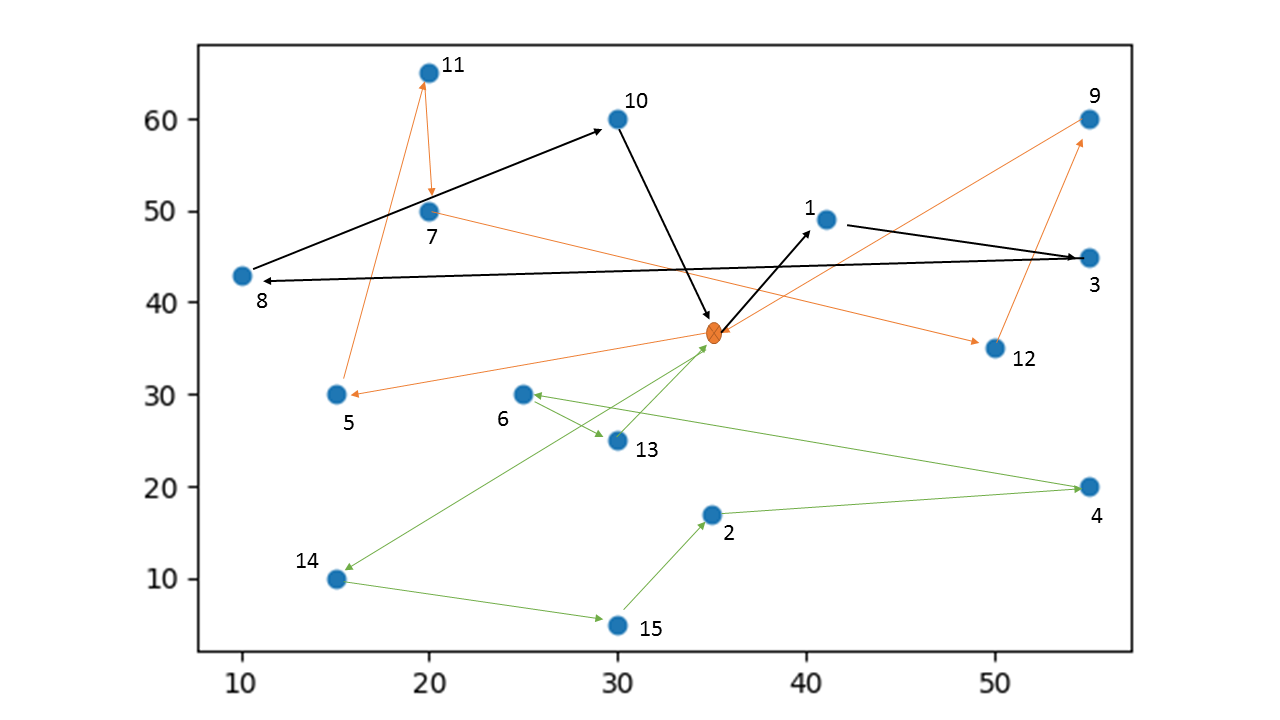
\includegraphics[width=150mm]{vrp.png}
    \caption{Mögliche, solide Lösung des VRP}  \label{Typen}
    {\footnotesize \textbf{orange:} Fahrzeug 1, \textbf{grün:} Fahrzeug 2, \textbf{schwarz:} Fahrzeug 3}
  \end{center}
\end{figure}

Es werden somit alle 15 Gene des Chromosoms bzw. alle 15 Kunden durch die drei verfügbaren Fahrzeuge abgedeckt, ohne dass dabei eine Restriktion gebrochen wird.
Um nun in Erfahrung zu bringen, wie effizient das vorliegende Chromosom ist in Bezug auf die Kosten, die es verursacht, ist, wird im genetischen Algorithmus eine Evaluation durchgeführt, mit der die Fitnessfunktion berechnet wird. 
Nur anhand dieser Fitnessfunktion ist es dem genetischen Algorithmus möglich, effizient zu selektieren und sich iterativ weiterzuentwickeln.


\subsubsection{Evaluation des Chromosoms im genetischen Algorithmus}

Der Evaluationsprozess ist dafür zuständig, die vorher bestimmte Fitnessfunktion zu berechnen und dadurch die Chromosome in der Population zu ordnen, um somit die Selektion für die nächste Generation einzuleiten.

In dieser Evaluation werden zunächst die jeweiligen Routen der einzelnen Fahrzeuge auf deren Kosten untersucht, im Anschluss zusammengeführt, wobei diese Summe schließlich den Nenner der Fitnessfunktion bildet:

\begin{center}
max F(x) = $\frac{1}{totalCost}$
\end{center}

Kostenverursachende Faktoren sind dabei sowohl die Wartezeiten, die eingegangen werden müssen, wenn das Fahrzeug zu früh beim Kunden ist als auch die Zeiten, die der Kunde auf seine Lieferung warten muss. 
Beide Kosten ergeben sich aus den Zeit- bzw. Distanzeinheiten, wobei beide Zeiten unterschiedlich gewichtet werden können. 
So ist es bspw. möglich, einer Verspätung beim Kunden deutlich mehr negative Auswirkungen zuzuschreiben, als dies beim Warten auf den Kunden der Fall ist, da bei Verspätungszeiten erhebliche Imageschäden für das Versandunternehmen entstehen könnten.

Kommt das Fahrzeug nun genau in dem Zeitfenster zwischen dem frühesten und spätesten Zeitpunkt beim Kunden an, so entstehen keinerlei Kosten, da weder auf den Kunden gewartet werden muss noch der Kunde auf die Lieferung warten muss.
Daraus lässt sich schließen, dass im Idealfall alle Kunden innerhalb ihres zur Verfügung stehenden Zeitraums angefahren werden sollten.

Beim ersten Kunden im Chromosom, dem Kunden 5, entstehen dabei nun Wartekosten i.H.v. 6.6922 Einheiten, da das Fahrzeug nach 20.61 Zeiteinheiten beim Kunden eintrifft, das Zeitfenster des Kunden allerdings erst bei 34 Zeiteinheiten öffnet.
Somit entsteht eine (hypothetische) Wartezeit i.H.v. 13.39 Zeiteinheiten und Wartekosten i.H.v. 6.6922 Einheiten, da diese mit dem Faktor 0.5 gewichtet werden. 

Deutlich kostenintensiver hingegen wird es beim Kunden 12 an der vierten Stelle der Route des ersten Fahrzeugs. 
Dieses kommt bei jenem Kunden erst zum Zeitpunkt 134.51 an, das Zeitfenster des Kunden schließt allerdings bereits zum Zeitpunkt 73.
Da Zeiteinheiten, die die Verspätung eines Fahrzeugs beim Kunden anzeigen, deutlich stärker gewichtet werden (Faktor 1.5), entstehen Kosten i.H.v. 92.26 Einheiten.
Nachdem die Route des ersten Fahrzeugs mit der Belieferung des Kunden 9 bzw. der Rückfahrt zum Depot abgeschlossen wird und die Zeitkosten dieser Route zusammengetragen wurden (193.98 Einheiten), werden im nächsten Schritt die Transportkosten berechnet.\\

Das erste Fahrzeug hat eine Strecke von 162.02 Distanzeinheiten zurückgelegt.
Diese Distanz wird nun mit dem Faktor multipliziert, der angibt, wie viel Kosten ein Fahrzeug pro gefahrene Distanzeinheit zurückgelegt (hier: 8).
Ergänzt wird dieses Produkt mit den Kosten für die Initialisierungskosten eines Fahrzeugs (hier: 60), sodass sich für diese Route des ersten Fahrzeugs Gesamtausgaben i.H.v. 1550.1659 Einheiten ergeben.

Werden diese Schritte für die Routen aller drei Fahrzeuge durch- bzw. zusammengeführt, so ergeben sich Gesamtkosten des Chromosoms i.H.v. 3959.7053 Einheiten.
Die Fitnessfunktion besitzt dann einen Wert von 0.0002525 und gibt dem Chromosom eine Fitness, die sich mit den anderen Chromosomen in der Population messen lässt.\\

Das zuvor betrachtete Chromosom war das beste aus einer Anfangspopulation, die dadurch zustande gekommen ist, dass Chromosome zufällig zusammengewürfelt wurden.
Für jedes einzelne wurde im nächsten Schritt die Fitness berechnet, wobei das Chromosom [5, 11, 7, 12, 9, 14, 15, 2, 4, 6, 13, 1, 3, 8, 10] mit dem Fitnesswert 0.0002525 am besten abschnitt und somit näher durchleuchtet wurde.

Nun besteht jedoch die Möglichkeit, dass dies bei weitem nicht das Chromosom ist, da es lediglich das beste Chromosom aus der zufällig generierten Anfangspopulation ist, die aus nicht mehr als 100 Chromosomen besteht, sodass dieses Chromosom eher einer heuristischen Lösung ähnelt.
Um dies herauszufinden, wurde in dieser Arbeit ein genetischer Algorithmus angewandt, für den bereits die Vorarbeit in Form der Generierung der Anfangspopulation geschaffen wurde.

\subsubsection{Crossover und Mutation}

Im nächsten Schritt wendet dieser Algorithmus in der ersten Iteration einen Crossover an, wodurch zwei zufällig gewählte Chromosome ausgewählt werden und auf eine zuvor festgelegte Art und Weise miteinander verknüpft werden, sodass am Ende zwei neue Chromosome entstehen, die wiederum in der Population mitaufgenommen werden.
Bei diesem Crossover kann es sich um die verschiedensten Methoden handeln, die jedoch meistens auf Zufallsprozessen basieren.
Der genetische Algorithmus, der in dieser Arbeit Anwendung fand, schnitt dabei eine bestimmte Sequenz aus dem Chromosom, bspw. [7, 12, 9] und addierte diese mit der kompletten Sequenz eines weiteren Chromosoms, sodass diese drei Gene dem zweiten, anderen Chromosom voran standen und in der Sequenz nun doppelt vorkamen. 
Die Doppelgänger in der nun künstlich verlängerten Sequenz wurden gestrichen, sodass wiederum ein völlig neues Chromosom entstanden ist.

Dieser Vorgang wird für einen bestimmten Anteil der Chromosome vorgenommen, wobei dieser Anteil durch die vorher bestimmte Crossover-Wahrscheinlichkeit bestimmt wird. 
In dieser Arbeit konnten mit einer Crossover-Wahrscheinlichkeit i.H.v. 0.7 die besten Ergebnisse erzielt werden, sodass aus der Anfangspopulation von 100 Chromosomen ca. 70 Chromosome 35 Chromosompaare bildeten, die wiederum 70 neue Chromosome erschaffen haben, sodass im Anschluss der ersten Iteration eine neue Population mit insgesamt 170 Chromosomen entstanden ist. 

Aus diesen 170 Chromosomen werden nun abermals mit einem Zufallsprozess die 100 überdurchschnittlich besten Chromosome mit in den nächsten Iterationsschritt mitaufgenommen, wobei darauf geachtet wird, dass mindestens der beste aus den 170 Chromosomen mit in diesen Schritt genommen werden, um die beste Lösung nicht zu verlieren und ggf. nicht noch einmal zu erhalten.\\ 

Bevor dieser finale Schritt innerhalb einer Iteration allerdings in die Wege geleitet wird, wird ein kleiner Bruchteil der Chromosome (hier: 1\%) nochmals mutiert, um zu gewährleisten, dass die Konvergenz des Algorithmus nicht zu früh eintritt und dieser sich u.U. in einem lokalen Minimum befindet. 
Auch hierbei existieren diverse Mutationsprozesse, die auf Zufallsmechanismen beruhen, wobei in dieser Arbeit auf einen Prozess zurückgegriffen wurde, der wiederum eine Sequenz des Chromosoms [7, 12, 9] herausschneidet und dieses an gleicher Stelle spiegelverkehrt [9, 12, 7] wieder einsetzt.\\

Nachdem 100 Iterationen mit einer Crossover- bzw. Mutations-Wahrscheinlichkeit i.H.v. 0.7 bzw. 0.01 bei einer Populationsgröße von 80 durchgeführt wurden, ergibt sich ein Chromosom, dass totale Kosten i.H.v. 3777.8872 verursacht und somit eine Fitness von 0.0002646 erreicht, was auch nach mehreren Durchläufen unerreicht bleibt und somit einen äußerst guten Wert darstellen sollte.
Das Chromosom nimmt dabei folgende Form an: 

\begin{center}
[5, 6, 13, 14, 15, 4, 3, 10, 11, 7, 8, 12, 1, 2, 9]
\end{center}

und verteilt sich dabei wie folgt auf die drei zur Verfügung stehenden Fahrzeuge: 

\begin{center}
Fahrzeug 1: 0 - 5 - 6 - 13 - 14 - 15 - 4 - 3 - 0

Fahrzeug 2: 0 - 10 - 11 - 7 - 8 - 12 - 1 - 0

Fahrzeug 3: 0 - 2 - 9 - 0
\end{center}

Auf Abbildung x ist zu sehen, dass sich die Verbindungslinien nun im Gegensatz zu denen in Abbildung x an keiner Stelle mehr durchkreuzen, was auch schon beim TSP ein Hinweis auf eine optimale Lösung ist.

\begin{figure}[h!]
  \begin{center}
    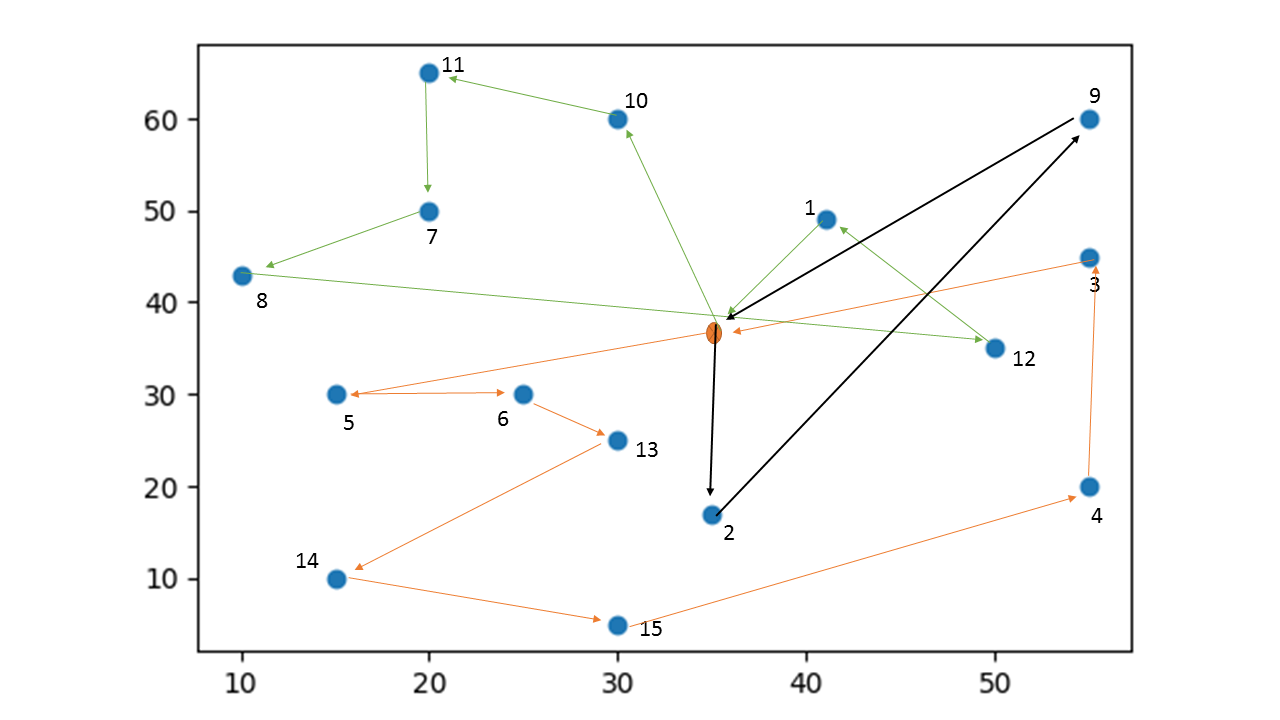
\includegraphics[width=150mm]{vrpOpt52.png}
    \caption{Optimale Lösung des VRP}  \label{Typen}
	{\footnotesize \textbf{orange:} Fahrzeug 1, \textbf{grün:} Fahrzeug 2, \textbf{schwarz:} Fahrzeug 3}
  \end{center}
\end{figure}




\newpage




\section{Schlussbemerkungen}
Zusammenfassung, kritische Würdigung, Ausblick\\\\
% Textteil: Ende

%%%%%%%%%%%%%%%%%%%%%%%%%%%%%%%%%%%%%%%%%%%%%%%%%%%%%%

Zum Schluss braucht man noch ein Literaturverzeichnis mit dem man im Text ganz einfach
zitieren kann, vgl.\cite{Det01}, \cite{OstSal04}, \cite{RieZimGla07}, \cite{SalPovNov08},
\cite{SchFlieBoy08} und \cite{ThaBosPet08}.

\newpage
\bibliographystyle{Prod_Seminar}    %legt die zu verwendende BIBTEX-Stildatei fest
\bibliography{Literatur}    %an der Stelle zu verwenden, an der das Literaturverzeichnis gesetzt werden soll;
                            %Literatur ist der Dateiname der BIB-Datei mit den Literatur-Informationen

\newpage
%%%%%%%%%%%%%%%%%%%%%%%%%%%%%%%%%%%%%%%%%%%%%%%%%%%%%%
%
%    ggf. Anhang
%
%%%%%%%%%%%%%%%%%%%%%%%%%%%%%%%%%%%%%%%%%%%%%%%%%%%%%%
\begin{appendix}
\section{aussagekräftige Überschrift für Inhalt des Anhangs}

\end{appendix}
%%%%%%%%%%%%%%%%%%%%%%%%%%%%%%%%%%%%%%%%%%%%%%%%%%%%%%
%
%   ENDE DES DOKUMENTS
%
%%%%%%%%%%%%%%%%%%%%%%%%%%%%%%%%%%%%%%%%%%%%%%%%%%%%%%

\end{document}
